%*****************************************
\chapter{Evaluation}\label{ch:evaluation}
%*****************************************
\label{eval}

In this chapter we investigate how the choice of image coding implementation affects bit error rates and capacity, and how the recipient group size affects codec performance. We also look at the effect of clearing the extension cache on page loading times and present some outcomes of the usability inspection.

Test data was generated on a laptop running Linux Mint 10.0 using a 1.46 Ghz Intel Pentium dual core CPU with 1 GiB of RAM. A 10 Mbpbs broadband connection was used to connect to the internet, with measured download/upload rates of around 8 Mbps and 2 Mbps respectively. For comparison, Firefox 4.0's minimum requirements include a single core 1.4 Ghz CPU with 512 MB of RAM \cite{firefox-req}. The average broadband speed in the UK is around 10 Mbps \cite{bband-stats}. 

\section{Image coding method}
\label{sec:imgcod}

We investigate how the concrete {\tt IConduitImage} implementation affects bit error rates and theoretical image capacity. The capacity puts a maximum limit on the number of possible recipients an image can be shared with, and also limits the size of the image being transmitted. In addition, error rates determine which error correction schemes are most suitable and what the final output error rate will be after application of a given scheme.

We test the hypothesis that the HWT, 3-bit scaling and 4-bit scaling methods provide both greater capacity and lower error rates than the naive methods described in Section \ref{ssec:naive} after undergoing Facebook's image upload process.

\subsection{Method}

In this instance, local simulation with {\tt libjpeg} was used since uploading to Facebook on this scale would be considerably time consuming and would possibly warrant account deletion due to violation of Facebook's terms. We compress over the quality factor interval 80-90; though it is most likely that Facebook uses IJG quality factor 85, this is only an estimate (see Appendix \ref{app:images}. This also means our results are somewhat robust to minor changes in Facebook's compression process.

We model the compression/decompression process as a binary symmetric channel and calculate the channel capacity for arbitrarily small error probability, using an empirically measured bit error rate as an estimate for the bit error probability.

Random input bytes are written to a $720 \times 720$ conduit image instance until full. The image is then saved as a JPEG at a given quality factor, reloaded and the data extracted. We record the Hamming distance between the input and output data. This process is repeated until the cumulative amount of data processed exceeds 1 GiB.

\begin{table}[tbph]
  \begin{center}
        \begin{tabular}{l l l l l}
        \textbf{Method} &\textbf{Bits per} &\textbf{Test set size} & \textbf{Test set size} &\textbf{Possible unique} \\ 
            &\textbf{block} &\textbf{(images)} &\textbf{(blocks)} &\textbf{blocks} \\ [0.1ex] \hline \\ [-1.5ex]
        Scaled3	&192	&5,523	&44,736,300	& $6.28 \times 10^{57}$ \\
        Scaled4	&256	&4,142	&33,550,200	& $1.16 \times 10^{77}$ \\
        Haar	&24	&44,186	&357,906,600	& $1.68 \times 10^{7}$ \\
        \end{tabular}
        \caption{Tabulated details of the testing process.}
        \label{tab:img-test}
    \end{center}
\end{table}

Table \ref{tab:img-test} summarises the number of useful bits each method can store in a single 64 x 8 bit greyscale JPEG luminance block along with the effective sample size and population size. Due to the number of samples the standard error is negligible, even before applying finite population correction where appropriate \footnote{In particular, for the Haar wavelet transform method the number of JPEG blocks encoded exceeds the number of unique data points that can be encoded in a single block.}. 

\subsection{Theoretical capacity calculation}
\label{ssec:capacity}

The per-image theoretical capacity $C$ is a function of the number of bits available per image $A$\footnote{Determined by the implementation.} and the bit error probability $p_e$:

\begin{equation}
    C = A \cdot (1 + H(p_e))
\end{equation}

where $H(x)$ is the binary entropy function. This provides the capacity in units of information per symbol, or in our case KiB per image.

\subsection{Results}

Both n-bit scaling methods showed marked improvements in error rates and capacity (see Figure \ref{graph:ber} and Figure \ref{graph:capacity}) in comparison to naive approaches.

The HWT method, however, had the lowest capacity of all methods tested. We attribute this mainly to the fact that two passes of the HWT were required to successfully reduce error rates, and that, due to the nature of the method, each pass reduces capacity by a factor of 4. The final error rates obtained do at least support the claim made in \cite{haar} that such an encoding scheme is reasonably immune to JPEG compression.


\begin{figure}[tbph]
  \begin{center}
\begin{tikzpicture}
    \begin{axis}[grid=major,xlabel=JPEG Quality Factor,ylabel=BER (\%), xmin=80, xmax=90,
    height=8cm,width=10cm,legend style={legend pos=outer north east}]
    \addplot
        table[x=QF,y=Sc3] {gfx/error_rate.data};
    \addplot
        table[x=QF,y=Sc4] {gfx/error_rate.data};
    \addplot[mark=diamond*, color=green]
        table[x=QF,y=Haar] {gfx/error_rate.data};
        
    \addplot[mark=triangle*, color=purple]
        table[x=QF,y=rgb] {gfx/error_rate0.data};
    \addplot[mark=diamond*, color=orange]
        table[x=QF,y=dct] {gfx/error_rate0.data};
    
    \legend{Scaled3,Scaled4,Haar,Pixels,DCT}
    \end{axis}
\end{tikzpicture}
    \caption{Bit error rate for varying quality factors.}
    \label{graph:ber}
  \end{center}
\end{figure}

\begin{figure}[tbph]
  \begin{center}
\begin{tikzpicture}

    \begin{axis}[grid=major,xlabel=JPEG Quality Factor,ylabel=Capacity (KiB/image), xmin=80, xmax=90,
    height=8cm,width=10cm,legend style={legend pos=outer north east }]
    \addplot
        table[x=QF,y=Sc3] {gfx/encoding_time.data};
    \addplot
        table[x=QF,y=Sc4] {gfx/encoding_time.data};
    \addplot[mark=|, color=green]
        table[x=QF,y=Haar] {gfx/encoding_time.data};
        
    \addplot[mark=triangle*, color=purple]
        table[x=QF,y=rgb2] {gfx/error_rate0.data};
    \addplot[mark=diamond*, color=orange]
        table[x=QF,y=dct2] {gfx/error_rate0.data};
        
    \legend{Scaled3,Scaled4,Haar,Pixels,DCT}
    \end{axis}
\end{tikzpicture}
    \caption{Per-image channel capacity (measured in KiB/image) for varying quality factors.}
    \label{graph:capacity}
  \end{center}
\end{figure}

\subsection{Implications}
\label{sec:cap:imp}

We can compare the capacity limit obtained in the previous section to the actual capacity achieved when an error correction scheme is applied (see Table \ref{tab:fec}).

We can also use the estimation of bit error probability to calculate the probability of decoder output error. Given the bit error probability $p$ we can obtain the symbol error probability $p_s$:

\begin{equation}
    p_s = 1 - (1-p)^m
\end{equation}

where $m$ is the number of bits per symbol. In general, for a Reed Solomon code with symbol error probability $p_s$ the decoded symbol error probability $p_s'$ is given by:

\begin{equation}
    p_s' = \frac{1}{2^m -1} \sum^{2^m - 1}_{i = t+1} i {{2^m - 1}\choose{i}} {p_s}^i (1-{p_s})^{2^m - 1 - i}
\end{equation}

where $t$ is the maximum number symbol errors we can correct \cite{rsfec-decode}. The resulting decoder output error rates, along with achievable capacity, are shown in Table \ref{tab:fec} for JPEG quality factor 85.

\begin{table}[tbph]
  \begin{center}
        \begin{tabular}{l l l l l l}
            
            \textbf{Method} & \textbf{FEC} & \textbf{$p$} & \textbf{$p_s$} & \textbf{$p_s'$} & \textbf{Capacity} \\  & &  &  &  & \textbf{(KiB)} \\[0.1ex] \hline \\ [-1.5ex]

            Haar & (15,9) & $4.20 \times 10^{-3}$ & $1.67 \times 10^{-2}$ & $2.47 \times 10^{-5}$ & 14.2 \\
            Haar &  (255,223) & $4.20 \times 10^{-3}$ & $3.31 \times 10^{-2}$ & $3.73 \times 10^{-4}$ & 20.8 \\
            Scaled3 & (15,9) & $8.30 \times 10^{-4}$ & $3.32 \times 10^{-3}$ & $4.28 \times 10^{-8}
$ & 113.9 \\
            \rowcolor{green!20!white} Scaled3 & (255,223) & $8.30 \times 10^{-4}$ & $6.62 \times 10^{-3}$ & $1.81 \times 10^{-13}
$ & 166.0 \\
            Scaled4 & (15,9) & $4.49 \times 10^{-2}$ & $1.68 \times 10^{-1}$ & $7.14 \times 10^{-1}$ & 151.9 \\
            Scaled4 & (255,223) & $4.49 \times 10^{-2}$ & $3.08 \times 10^{-1}$ & $3.08
 \times 10^{-1}$ & 221.4 \\
            
        \end{tabular}
        \caption{Bit error probability, symbol error probability and output symbol error probability for each possible combination.}
        \label{tab:fec}
    \end{center}
\end{table}

The 4-bit scaling class results in error rates too large to be corrected with the Reed Solomon codes used here, indicating that a different FEC scheme would be appropriate.

Using the 3-bit scaling class along with (255,223) FEC codes (highlighted in green) we would expect less than one bit error in a terabyte of encoded data. For comparison, this approaches hard disk drive read error rates \footnote{Stated by at least one hard drive vendor to be 1 uncorrectable read error in $10^{14}$ bits, or 10 terabytes \cite{hdd-errors}.}. The capacity (approximately 165 KiB) is also within 10\% of the Shannon limit for 3-bit scaling. We focus on this combination for the remainder of the evaluation.



\FloatBarrier
\section{Recipient group size}
\label{sec:recsize}

We investigate how recipient group size affects encoding and decoding performance. Large or highly variable decoding times would have an adverse effect on usability, in particular since decoding is triggered automatically whilst browsing. Potentially, practical recipient group sizes might be limited due to performance issues.

\begin{figure}[tbph]
    \begin{center}
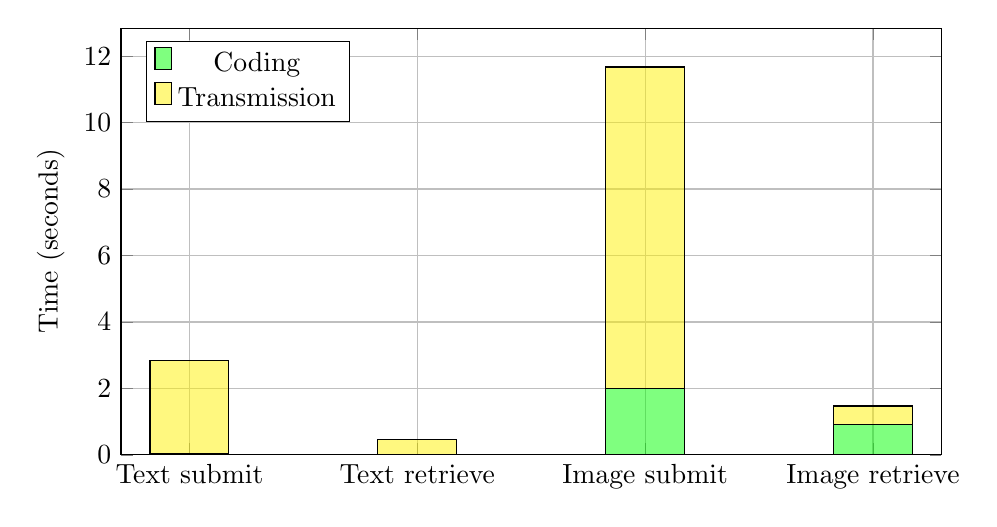
\begin{tikzpicture}
\begin{axis}[grid=major,ybar stacked, 
    symbolic x coords={Text submit,Text retrieve, Image submit, Image retrieve},
    xtick=data,ylabel=Time (seconds), width=12cm, height=7cm,
    legend style={legend pos=north west, area legend},
    bar width=1cm, ymin=0]

    \addplot[fill=green, fill opacity=0.5] coordinates
        {(Text submit,0.0444) (Text retrieve,0.0172) (Image submit,2.0074) (Image retrieve,0.9044)};
    \addplot[fill=yellow, fill opacity=0.5] coordinates
        {(Text submit,2.8013) (Text retrieve,0.4446) (Image submit,9.6655) (Image retrieve,0.5662)};
    \legend{Coding,Transmission}

\end{axis}
\end{tikzpicture}
    \caption{Average timing results for a 10,000 character note and an (approximately) 50 KiB image.}
    \label{graph:txt-sync}
  \end{center}
\end{figure}

Preliminary tests (see Figure \ref{graph:txt-sync}) show that time spent encoding and decoding text is too short to be an issue in any case. Therefore, we test the hypothesis that recipient group size has an  effect on image codec performance and measure the extent of this effect.



\subsection{Method}

A 50 KiB random test image was encrypted using 248-bit AES and 2048-bit RSA, encoded into a lossless image format.\footnote{Using 3-bit scaling and (255,223) Reed Solomon codes.} For each test the number of recipients was increased, from 1 up to a maximum of 400. Recipients were duplicates and selected at random from a pool of 15. The image was then compressed using {\tt libjpeg} and the data deciphered. Encode and decode times were recorded and included writing to and from disk but not JPEG compression. Checks were made to ensure that no decode errors occurred.

\subsection{Results}

\begin{figure}[tbph]
    \begin{center}
    
\begin{tikzpicture}
\begin{axis}[grid=major,
    xlabel=Recipient group size, ylabel=Encoding Time (seconds), height=10cm,width=10cm,
    ymin=0, xmin=0, xmax=400, legend style={legend pos=south west, empty legend}]
    
    \addplot[only marks, mark=x] table[x=r,y=t]
        {gfx/submit.data};
    \addplot[no marks, color=red] table[x=r,y={create col/linear regression={y=t}}]
        {gfx/submit.data};
    \addlegendentry{Slope = $\pgfmathprintnumber{\pgfplotstableregressiona}$};
    \addlegendentry{R = $\pgfmathprintnumber{0.726}$}

\end{axis}
\end{tikzpicture}

\begin{tikzpicture}
\begin{axis}[grid=major,
    xlabel=Recipient group size, ylabel=Decoding Time (seconds), height=10cm,width=10cm,
    ymin=0, xmin=0, xmax=400, legend style={legend pos=south west, empty legend}]
    
    \addplot[only marks,mark=x] table[x=r,y=t]
        {gfx/retrieve.data};
    \addplot[no marks, color=red] table[x=r,y={create col/linear regression={y=t}}]
        {gfx/retrieve.data};
    \addlegendentry{Slope = $\pgfmathprintnumber{\pgfplotstableregressiona}$};
    \addlegendentry{R = $\pgfmathprintnumber{0.615}$}

\end{axis}
\end{tikzpicture}

    \caption{Encoding (top) and decoding (bottom) times as recipient numbers increase.}
    \label{graph:subrep}
  \end{center}
\end{figure}

The results in Figure \ref{graph:subrep} show a significant linear correlation between group size and codec performance ($p < 0.001$). For both decoding and encoding, a group size of 400 incurs an average time overhead of less than 8\% compared to a single recipient.


\subsection{Implications}

Given a group size of $n$ and public key size $p$ the transmission overhead, in bytes, is given by:

\begin{equation}
    (n \times (4 + p)) + 16
\end{equation}

The implementation used for testing has a capacity of 165 KiB, which must include both the transmission overhead and the image itself. Thus group sizes larger than 400 are already approaching the capacity limit. Even given increased capacity, our results show that performance issues are unlikely to be the limiting factor to recipient group sizes.


\section{Plaintext caching}
\label{sec:ptextc}

Due to the nature of the parsing process (see Section \ref{ssec:proc-targets}) a cache of plaintext content accumulates on the user's machine. This cache can be cleared to decrease storage utilisation or for security purposes\footnote{Specific attacks involving the cache are not included in our initial threat model since they involve a malfeasor having access to the user's machine, a scenario which is considered a threat in itself.}, though this is likely to have a negative effect on response times and therefore on usability.

We test the hypothesis that clearing the plaintext cache increases page load times and estimate the worst case increase.


\subsection{Method}

Sample news feeds were generated with 15 encrypted status update entries, as this is the number of news feed entries Facebook first loads \footnote{More are loaded dynamically when the user scrolls to the bottom of the page.}. Status update messages were random ASCII text 420 characters in length, the maximum permitted. The pages were loaded repeatedly 400 times, ensuring that both the browser cache and extension cache were cleaned after each load.

The entire process was then repeated for a news feed containing 15 image objects, once again random images of size 50 KiB, instead of status messages. A second set of tests were performed without cleaning the extension cache (which was preloaded with the page's content).

The start time of each test was logged, along with the subsequent load times of the encrypted objects. 

    \begin{figure}[tbph]
        \begin{center}
                
\includegraphics[width=10cm]{screens/parrots1.png}
                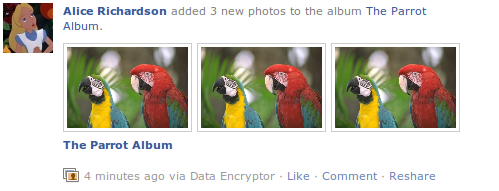
\includegraphics[width=10cm]{screens/parrots2.png}
            \caption{News feed excerpt containing encrypted image thumbnails, before (top) and after (bottom) parsing.}
            \label{scn:parrots}
        \end{center}
    \end{figure}


\subsection{Results}

The effect of plaintext caching on the overall page loading times can be seen in Figure \ref{graph:hist}. On average, load times for the entire page and all encrypted items were increased roughly by a factor of 2 for the feed containing just text and by a factor of 5 for the feed containing images. 

\begin{figure}[tbph]
    \begin{center}
\begin{tikzpicture}
\begin{axis}[xlabel=Time (seconds), ylabel=Frequency,
grid=major,const plot, ymin=0, enlargelimits=false,
width=12cm, height=5cm, legend style={area legend}]

    \addplot[fill=blue, fill opacity=0.5] table[x=t,y=Text] {gfx/async_text_hist.data};
    
    \addplot[fill=red, fill opacity=0.5] table[x=t,y=Text_c] {gfx/async_text_hist.data};
    
    \addplot+[sharp plot,blue, mark=no marker] coordinates
        {(6.403,0) (6.403,56)};
        
    \addplot+[sharp plot,red, mark=no marker] coordinates
        {(3.463,0) (3.463,56)};
    
    \legend{Cache off,Cache on}
\end{axis}
\end{tikzpicture}

\begin{tikzpicture}
\begin{axis}[xlabel=Time (seconds), ylabel=Frequency,
grid=major,const plot, ymin=0, enlargelimits=false,
width=12cm, height=5cm, legend style={area legend}]
    
    \addplot[fill=blue, fill opacity=0.5] table[x=t,y=Images] {gfx/async_image_hist.data};
    
    \addplot[fill=red, fill opacity=0.5] table[x=t,y=Images_c] {gfx/async_image_hist.data};
    
    \addplot+[sharp plot,blue, mark=no marker] coordinates
        {(19.169,0) (19.169,130)};

    \addplot+[sharp plot,red, mark=no marker] coordinates
        {(4.067,0) (4.067,130)};
    
    \legend{Cache off,Cache on}
    
\end{axis}
\end{tikzpicture}
    \caption{Histogram of 400 page loading times for news feeds containing 15 encrypted messages (top) and 15 encrypted images (bottom).}
    \label{graph:hist}
  \end{center}
\end{figure}

After the first item has loaded we can also look at the subsequent waiting time between loads. The most dramatic increase is for images, as seen in Table \ref{tab:async}.

\begin{table}[tbph]
  \begin{center}
        \begin{tabular}{+l ^l ^l ^l ^l}
            \rowstyle{\bfseries}%
            Element & \multicolumn{2}{^l}{Text (ms)} & \multicolumn{2}{^l}{Image (ms)}  \\
            \midrule 
            2 &	    30.6 &	2.6 &	782.3 &	6.5 \\
            3 &	    53.9 &	2.3 &	752.0 &	6.5 \\
            4 &	    29.0 &	2.3 &	761.6 &	6.4 \\
            5 &	    48.3 &	2.3 &	757.8 &	6.3 \\
            6 &	    48.9 &	2.3 &	781.0 &	6.4 \\
            7 &	    62.4 &	2.3 &	755.8 &	6.4 \\
            8 &	    113.4 &	2.4 &	769.8 &	6.5 \\
            9 &	    162.4 &	2.3 &	763.6 &	6.5 \\
            10 &    60.0 &	2.2 &	752.5 &	6.4 \\
            11 &    52.8 &	2.3 &	623.2 &	6.5 \\
            12 &    60.0 &	2.3 &	928.3 &	6.5 \\
            13 &    62.3 &	2.3 &	698.8 &	6.4 \\
            14 &    57.1 &	2.4 &	715.2 &	6.4 \\
            15 &    116.5 &	2.4 &	376.0 &	6.4
        \end{tabular}
        \caption{Page load times with (left column) and without (right column) cache cleansing beforehand.}
        \label{tab:async}
    \end{center}
\end{table}


\subsection{Implications}

Currently the plaintext cache is wiped on initialisation and destruction. Based on our results, most users would likely benefit from lengthening the cache expiration period, unless the extension was used mainly for text communications rather than image sharing. A full study of how the cache increases in size over time would required to make this judgement however; this was unfortunately not possible in the limited evaluation timeframe.





\FloatBarrier
\section{Usability inspection}
\label{sec:cw}

We present the final outcome of the usability inspection that was used as part of the development process. For the sake of concision we evaluate only the submission process for comments and images, as these contain the longest sequences of actions required of a user. The full set of tests is included in Appendix \ref{app:cw}.

We test the hypothesis that a typical Facebook user can successfully share an encrypted image, and that a similar user can successfully submit to that image an encrypted comment.


\subsection{Method}

We use the cognitive walkthrough (as described by Wharton et al \cite{cogwalk}) to evaluate the success of the user interface. This section consists of two of the final success stories and a defence of their validity. They refer to claims demonstrated by other walkthroughs which can be found Appendix \ref{app:cw}.

We only consider one class of user - a typical Facebook user who is therefore familiar with the Facebook user interface. It is therefore assumed that actions such as "navigate to a given friend's profile" can be performed without additional aid. It is also assumed that the user will follow their usual actions when trying to perform an encrypted operation - when trying to upload an encrypted image they will, for example, simply follow the normal procedure for uploading an image rather than searching for some hidden option. Finally, we make the assumption that the extension has been installed and enabled and that the toolbar has not been hidden.


\subsection{Uploading an encrypted image}
A user wishing to send an encrypted image to 405 friends who also have the extension, does so.

\begin{desc}

    \item[Action Sequence] \hfill
    \begin{enumerate}
        \item Add any public keys required.
        \item Navigate to the image upload page for the required album (see Figure \ref{scn:pic-up}).
        \item Select the image to encrypted.
        \item Check the {\tt [Encrypt]} check box.
        \item Click the {\tt [Submit]} button.
        \item Use the friend selector to select recipients and submit.
    \end{enumerate}
    
    \item[Defence of Credibility] \hfill
        \begin{itemize}
            
            \item The user knows he must add public keys of recipients beforehand and how to do so. If the user has no public keys Appendix \ref{app:cw:addkey} demonstrates that he will be able to add one of his intended recipients. Since the process is reasonably simple - simply navigate to their page and click a clearly marked button, we assume that any user who has performed it once can do so again if they wish, without further instruction. The link between adding public keys and being able to choose those friends as recipients should be fairly obvious; when the first key is added and encryption attempted again that same friend will appear as the only possible recipient.
            
            \item Facebook user will be familiar with the process of uploading an image. We assume a user trying to upload an encrypted image will be likely to try the method they are already familiar with.
            
            \item User knows things are OK since he sees the encryption check box option on arriving at the upload page. Check box leaves little room for confusion over whether an upload will or won't be encrypted.
            
            \item User knows to select an image to upload since the process is identical to uploading plaintext images.
            
            \item User knows to select {\tt [Encrypt]} check box since uploading an encrypted image is the original task.
            
            \item User knows things are OK since the recipient selector pops up.
            
            \item User knows how to use the recipient selector (see Appendix \ref{app:cw:sel}).
            
            \item User knows things are OK as Facebook handles the upload process from here as per normal, notifying user when the upload is complete.
            
        \end{itemize}
    
\end{desc}


    \begin{figure}[tbph]
        \begin{center}
        
                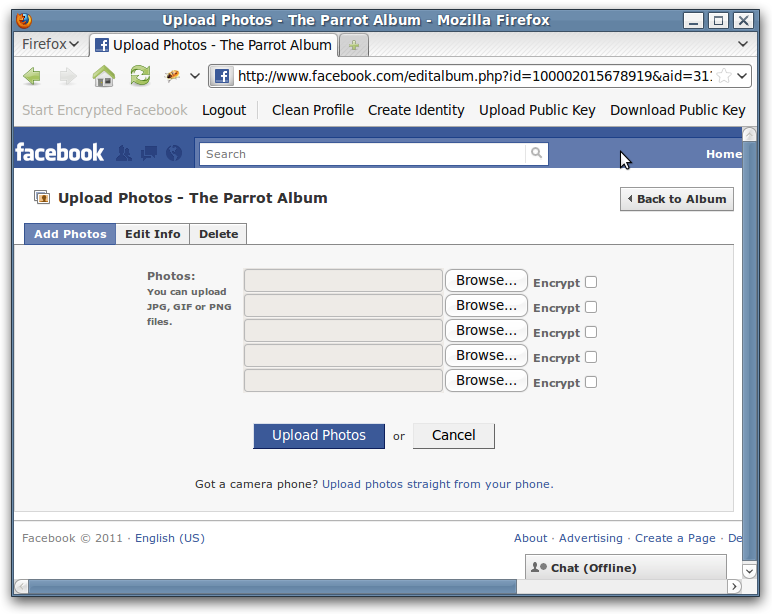
\includegraphics[width=12cm]{screens/pic-upload.png}

            \caption{Input fields and controls for submitting encrypted images.}
            \label{scn:pic-up}
        \end{center}
    \end{figure}


\subsection{Posting a comment}
A user has navigated to his news feed. He wishes to write an encrypted reply to a plaintext comment on a news feed post of an encrypted photo. It is assumed he already possesses the public keys required and can decrypt the photo in question.

\begin{desc}

    \item[Action Sequence] \hfill
    \begin{enumerate}
        \item Select the comment box below the plaintext reply.
        \item Type comment in plaintext.
        \item Click the {\tt [Encrypt \& Submit]} button.
        \item Use the friend selector to select recipients and submit.
        \item Refresh the page to review comment.
    \end{enumerate}
    
    \item[Defence of Credibility] \hfill
        \begin{itemize}
            
            \item User knows to select the comment box. This is required for submitting a plaintext comment, we assume the user will try the method they are used to.
            
            \item User knows things are OK as the {\tt [Encrypt \& Submit]} appears once the textbox has focus.
            
            \item User knows to type in the comment - this is identical to submitting a plaintext comment.
            
            \item User knows to click {\tt [Encrypt \& Submit]}. The user is familiar with clicking a similar submit button during plaintext entry. The button is positioned beside the {\tt [Submit]} for plaintext entry, is styled like the {\tt [Submit]} button and is clearly labelled. Submitting an encrypted comment is part of the original task.
            
            \item User knows how to use the recipient selector (see Appendix \ref{app:cw:sel}).
            
            \item User knows things are OK as Facebook handles the submission process from here as per normal. A loading icon appears briefly, then the comment itself appears.
            
            \item User knows that their submission was encrypted as this fact is stated as part of the comment encoding.
            
            \item User knows they must refresh the page to view their own comment. Even if this is their first encrypted submission, Facebook users will be familiar with the process of refreshing a page when something is not working or to view an update. If the user does not make the connection right away, they should realise that encrypted text submissions are decrypted as a page first loads when they return to the page and see the item decrypted automatically.
        
        \end{itemize}
\end{desc}


    \begin{figure}[tbph]
        \begin{center}
        
                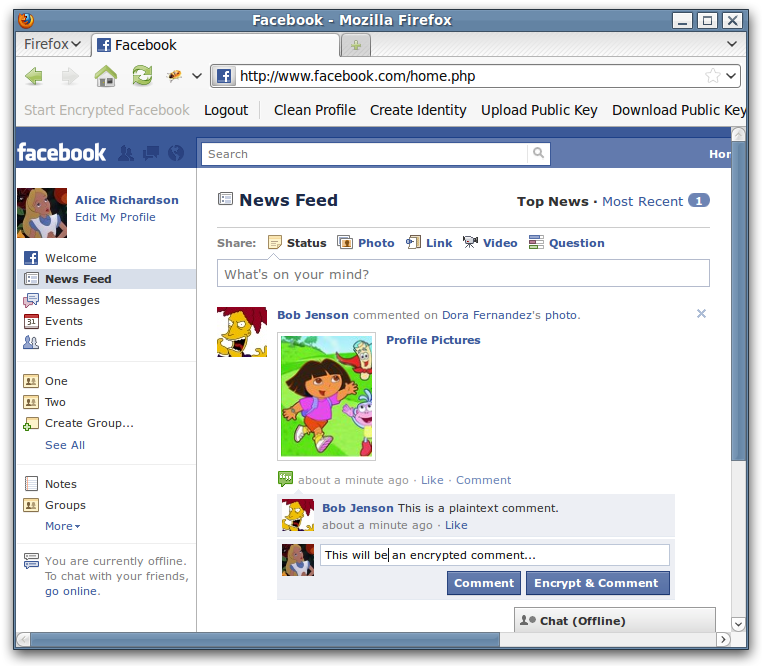
\includegraphics[width=12cm]{screens/comment.png}

            \caption{Input fields and controls for posting a comment to a news feed entry.}
            \label{scn:comment}
        \end{center}
    \end{figure}